%******************************************************************************%
% Copyright (C) 2018  Louis Solofrizzo                                         %
%                                                                              %
% This content is considered a free software: you can redistribute it          %
% and/or modify it under the terms of the GNU General Public License as        %
% published by the Free Software Foundation, either version 3 of the License,  %
% or (at your option) any later version.                                       %
%                                                                              %
% This program is distributed in the hope that it will be useful,              %
% but WITHOUT ANY WARRANTY; without even the implied warranty of               %
% MERCHANTABILITY or FITNESS FOR A PARTICULAR PURPOSE.  See the                %
% GNU General Public License for more details.                                 %
%                                                                              %
% You should have received a copy of the GNU General Public License            %
% along with this program.  If not, see <https://www.gnu.org/licenses/>.       %
%******************************************************************************%

%******************************************************************************%
%                                                                              %
%                          KFS_3.en.tex for KFS_3                              %
%                                                                              %
%                  Created on : Wed May 30 13:37:00 2016                       %
%          Made by : Louis "Ne02ptzero" Solofrizzo <louis@ne02ptzero.me>       %
%                                                                              %
%******************************************************************************%

\documentclass{42-en}


%******************************************************************************%
%                                                                              %
%                                    Header                                    %
%                                                                              %
%******************************************************************************%
\begin{document}


                           \title{KFS\_3}
                          \subtitle{Memory}
                       \member{Louis Solofrizzo}{louis@ne02ptzero.me}
                        \member{42 Staff}{pedago@42.fr}

\summary {
	The sweet world of memory
}

\maketitle

\tableofcontents

\newpage
%******************************************************************************%
%                                                                              %
%                                  Foreword                                    %
%                                                                              %
%******************************************************************************%
\chapter{Foreword}
	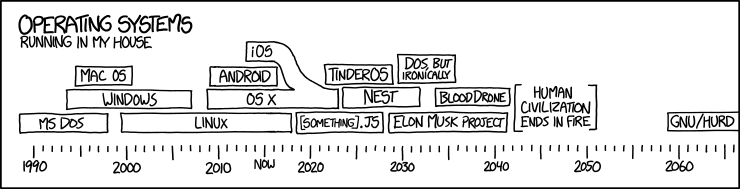
\includegraphics[width=16cm]{./operating_systems.png}
	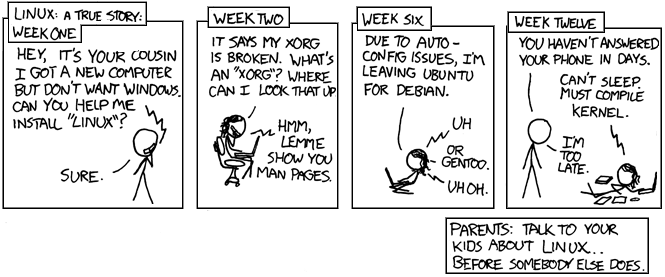
\includegraphics[width=16cm]{./cautionary.png}
	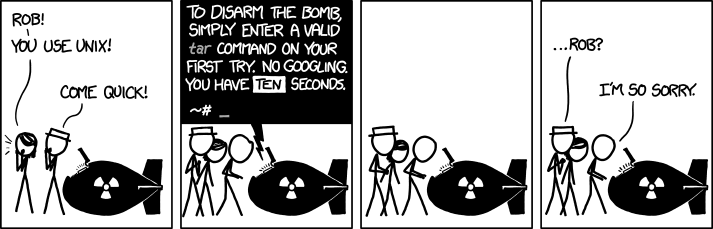
\includegraphics[width=16cm]{./tar.png}


%******************************************************************************%
%                                                                              %
%                                 Introduction                                 %
%                                                                              %
%******************************************************************************%
\chapter{Introduction}

	\section{Foreword}
	Welcome to \texttt{Kernel from Scratch}, third subject. This time, we will
	make a proper memory !\\

	In the last subject, you have declared your memory space to the
	\texttt{BIOS}, and now it's the time to use it. In other words, you will code
	\texttt{memory paging}, \texttt{allocation}, and \texttt{free}.\\

	First, let's take a look of what a dynamic memory allocation is:
	\begin{quotation}
		\textit{The task of fulfilling an allocation request consists of
		locating a block of unused memory of sufficient size. Memory requests
		are satisfied by allocating portions from a large pool of memory called
		the heap or free store. At any given time, some parts of the heap are
		in use, while some are "free" (unused) and thus available for future
		allocations.}
	\end{quotation}

	I'm sure you all know how to use a \texttt{malloc}, and what's behind it.
	But this subject is more than a \texttt{malloc}, it's about
	\texttt{memory paging}, the difference between \texttt{physical} and
	\texttt{virtual} memory, and memory code structures.\\

	This subject is one of the more important of the \texttt{Kernel from Scratch}
	series.	Take your time, write proper code, cause if you don't, you will
	regret it !

\newpage

	\section{Theory}
	Note: This section is from the \texttt{Samy Pesse}'s book:
	\href{https://www.gitbook.com/book/samypesse/how-to-create-an-operating-system/details}
	{How to write an operating system}. A must read !
	\subsection{Why do we need paging ?}
	Paging will allow your \texttt{kernel} to:

	\begin{itemize}\itemsep1pt
		\item Use the hard-drive as a memory and not be limited by the machine
		ram memory limit
		\item To have a \texttt{unique} memory space for each process
		\item To allow and unallow memory space in a \texttt{dynamic} way
	\end{itemize}

	In a \texttt{paged} system, each process may execute in its own \texttt{4gb}
	area of memory, without any chance of effecting any other process's memory,
	or the kernel's.\\
	It simplifies multitasking.\\
	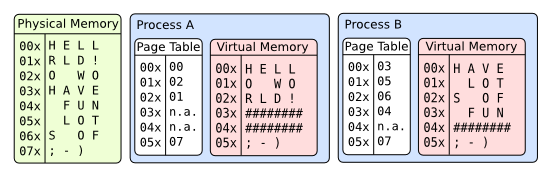
\includegraphics[width=16cm]{./processes.png}

	\subsection{How does it work ?}
	The translation of a linear address to a physical address is done
	in multiple steps:

	\begin{itemize}\itemsep1pt
		\item The processor use the registry \texttt{CR3} to know the physical
		address of the pages directory.
		\item The \texttt{first} 10 bits of the linear address represent
		an \texttt{offset} (between 0 and 1023), pointing to an entry
		in the pages directory. This entry contains the physical address
		of a pages table.
		\item The \texttt{next} 10 bits of the linear address represent an
		\texttt{offset}, pointing to an entry in the pages table. This entry
		is pointing	to a \texttt{4ko} page.
		\item The \texttt{last} 12 bits of the linear address represent an
		\texttt{offset} (between 0 and 4095), which indicates the position
		in the \texttt{4ko}	page.
	\end{itemize}
	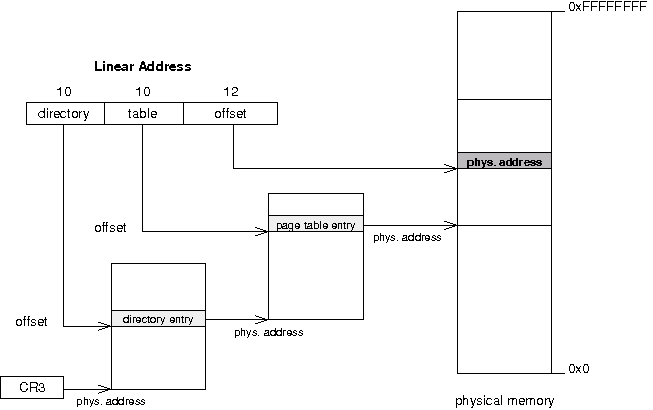
\includegraphics[width=16cm]{./paging_memory.png}

\newpage

	\subsection{Format for pages table and directory}
	The two types of entries (table and directory) look like the same.
	Only the field in gray will be used in the \texttt{kernel}.\\
	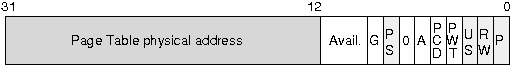
\includegraphics[width=16cm]{./page_directory_entry.png}

	\begin{itemize}\itemsep1pt
		\item \texttt{P}: indicate if the page or table is in physical memory
		\item \texttt{R/W}: indicate if the page or table is accessible in
		writting (equals 1)
		\item \texttt{U/S}: equals 1 to allow access to non-preferred tasks
		\item \texttt{A}: indicate if the page or table was accessed
		\item \texttt{D}: (only for pages table) indicate if the page was written
		\item \texttt{PS}: (only for pages directory) indicate the size of pages :
		\begin{itemize}\itemsep1pt
			\item 0 = 4kb
			\item 1 = 4mb
		\end{itemize}
	\end{itemize}

	Notes: Physical addresses in the pages directory or pages table are written
	using 20 bits because these addresses are aligned on 4kb, so the last 12bits
	should be equal to 0.

	\begin{itemize}\itemsep1pt
		\item A pages directory or pages table used 1024*4 = 4096 bytes = 4k
		\item A pages table can address 1024 * 4k = 4 Mb
		\item A pages directory can address 1024 (1024 4k) = 4 Gb
	\end{itemize}


\newpage
%******************************************************************************%
%                                                                              %
%                                  Goals                                       %
%                                                                              %
%******************************************************************************%
\chapter{Goals}

	At the end of this subject, you will have:
	\begin{itemize}\itemsep1pt
		\item A complete memory code structure, with pagination handling
		\item Read and Write rights on memory
		\item User space memory and Kernel space memory
		\item Physical and Virtual memory
		\item Code helpers for physical memory, like \texttt{kmalloc},
		\texttt{kfree}, \texttt{ksize}, \texttt{kbrk}
		\item Code helpers for virtual memory, like \texttt{vmalloc},
		\texttt{vfree}, \texttt{vsize}, \texttt{vbrk}
		\item Kernel Panic handling
	\end{itemize}
	
	Lot of work on this one !

\newpage
%******************************************************************************%
%                                                                              %
%                             General instructions                             %
%                                                                              %
%******************************************************************************%
\chapter{General instructions}
	\section{Code and Execution}
		\subsection{Emulation}
		The following part is not mandatory, you're free to use any virtual
		manager you want to, however, i suggest you to use \texttt{KVM}.
		It's a \texttt{Kernel Virtual Manager}, and have advanced execution
		and debugs functions.
		All of the example below will use \texttt{KVM}.
		\subsection{Language}
			The \texttt{C} language is not mandatory, you can use any language
			you want for this suit of projects.\\
			Keep in mind that all language are not kernel friendly, you could
			code a kernel with \texttt{Javascript}, but are you sure
			it's a good idea ?\\ Also, a lot of the documentation are
			in \texttt{C}, you will have to 'translate' the code all along
			if you choose a different language.\\

			Furthermore, all of the features of a language cannot be used in a
			basic kernel. Let's take an example with \texttt{C++} :\\
			This language uses 'new' to make allocation, class and structures
			declaration. But in your kernel, you don't have a memory interface
			(yet), so you can't use those features now.\\

			A lot of language can be used instead of \texttt{C},
			like \texttt{C++}, \texttt{Rust}, \texttt{Go}, etc.
			You can even code your entire kernel in \texttt{ASM} !\\
			\begin{center}
			  
\includegraphics[width=8cm]{choose.jpg}
			\end{center}

\newpage


	\section{Compilation}
		\subsection{Compilers}
			You can choose any compilers you want. I personnaly use	\texttt{gcc}
			and \texttt{nasm}. A Makefile must be turn in to.
		\subsection{Flags}
			In order to boot your kernel without any dependencies, you must compile
			your code with the following flags (Adapt the flags for your language,
			those ones are a \texttt{C++} example):
			\begin{itemize}\itemsep1pt
				\item \texttt{-fno-builtin}
				\item \texttt{-fno-exception}
				\item \texttt{-fno-stack-protector}
				\item \texttt{-fno-rtti}
				\item \texttt{-nostdlib}
				\item \texttt{-nodefaultlibs}
			\end{itemize}
			Pay attention to \texttt{-nodefaultlibs} and \texttt{-nostdlib}.
			Your Kernel will be compiled on a host system, yes, but cannot be
			linked to any existing library on that host, otherwise it will not
			be executed.
	\section{Linking}
		You cannot use an existing linker in order to link your kernel.
		As written above, your kernel will not boot. So, you must create a linker
		for your kernel.\\
		Be carefull, you \texttt{CAN} use the 'ld' binary available on your host,
		but you \texttt{CANNOT} use the .ld file of your host.
	\section{Architecture}
		The \texttt{i386} (x86) architecture is mandatory
		(you can thank me later).
	\section{Documentation}
		There is a lot of documentation available, good and bad.
		I personnaly think the \texttt{\href{http://wiki.osdev.org/Main_Page}
		{OSDev}} wiki is one of the best.
	\section{Base code}
		In this subject, you have to take your precedent \texttt{KFS} code,
		and work from it !\\ Or don't. And rewrite all from scratch. Your call !

\newpage
%******************************************************************************%
%                                                                              %
%                             Mandatory part                                   %
%                                                                              %
%******************************************************************************%
\chapter{Mandatory part}

	You must implement a \texttt{complete}, \texttt{stable} and \texttt{functionnal}
	memory system in your kernel.\\
	Let's follow this task, point by point:
	\begin{itemize}\itemsep1pt
		\item You must enable memory paging in your \texttt{Kernel}
		\item You must code a memory structure that handle paging and memory
		rights (Careful, you don't have the tools yet to know who's accessing
		the memory, so all of this is theoric at the moment)
		\item You must define \texttt{Kernel} and \texttt{User space}
		\item You must implement a function to \texttt{create} / \texttt{get}
		memory pages
		\item You must implement functions to \texttt{allocate}, \texttt{free}
		and \texttt{get} size of a variable.
		\item You must implement those functions for \texttt{virtual} and
		\texttt{physical} memory
		\item You must handle "\texttt{kernel panics}" (Print, stop the kernel)
		\item Your work should not exceed 10 MB.
	\end{itemize}

	Some notes:\\
	First, about this implementation. If you remember correctly, in the first subject,
	i was speaking about language (Other than \texttt{C}) limitation,
	and memory integration.
	Now's the time to implement it !\\
	Secondly, about the panics. There are some times when the kernel must stop,
	and some times when the kernel can continue. So all panics are not fatal,
	make the difference.

\newpage
%******************************************************************************%
%                                                                              %
%                                 Bonus part                                   %
%                                                                              %
%******************************************************************************%
\chapter{Bonus part}

	Since this subject is really, really hard, the bonuses are not really important.\\
	Try to focus on the code itself, because the memory is most important
	part of your kernel, by far. But if you are looking for some things to do
	after that, try to implement \texttt{memory dumping} and \texttt{debug}
	in the last "mini-shell" subject.
	Keep in mind that will be not graded.

\newpage
%******************************************************************************%
%                                                                              %
%                           Turn-in and peer-evaluation                        %
%                                                                              %
%******************************************************************************%
\chapter{Turn-in and peer-evaluation}

	Turn your work into your \texttt{GiT} repository, as usual.
	Only the work present on your repository will be graded in defense.\\

	Your must turn in your code, a Makefile and a basic virtual image for your kernel.\\
	Side note about that image, your kernel does nothing with it yet,
	SO THERE IS NO NEED TO BE SIZED LIKE AN ELEPHANT.




%******************************************************************************%
\end{document}
